\subsection*{Amortización y depreciación}
\addcontentsline{toc}{subsection}{Amortización y depreciación}

\subsubsection*{Préstamo}
\addcontentsline{toc}{subsubsection}{Préstamo}

Para iniciar el proyecto, se adquirió un préstamo con una entidad bancaria, el cual se sumó al aporte social realizado por los socios. En la tabla \ref{Prestamo} se presenta la información correspondiente al préstamo destinado a la inversión en los activos fijos iniciales del proyecto, así como las condiciones bajo las cuales fue otorgado.

\begin{table}[H]
	\centering
	\caption[{Préstamo}]{\centering Tabla de préstamo bancario. \textit{Fuente:} Autores.}
	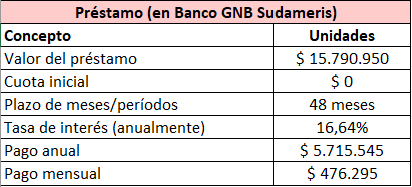
\includegraphics[width=11cm]{Imagenes/Prestamo.png}
	\label{Prestamo}
\end{table}

\subsubsection*{Amortización}
\addcontentsline{toc}{subsubsection}{Amortización}

A continuación, se presenta un resumen del pago realizado de forma anual. En la tabla se evidencia la amortización total de la deuda, la cual se proyecta para un período de cuatro años. De esta manera, se puede observar cómo se realizará el pago de la deuda dentro del período de tiempo establecido y cuál será el saldo final hasta alcanzar un valor de 0, teniendo en cuenta los intereses generados por el préstamo.

\begin{table}[H]
	\centering
	\caption[{Amortización}]{\centering Tabla de la amortización. \textit{Fuente:} Autores.}
	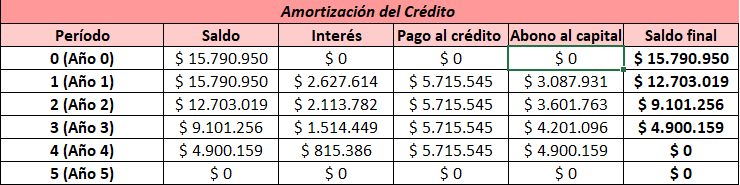
\includegraphics[width=13cm]{Imagenes/Amortizacion.png}
	\label{Amortizacion}
\end{table}

\subsubsection*{Depreciación}
\addcontentsline{toc}{subsubsection}{Depreciación}

En la tabla \ref{Depreciacion} se presenta la maquinaria que será utilizada en el proyecto, junto con el cálculo de su depreciación, considerando tanto el desgaste por uso como la obsolescencia de los dispositivos. Se estima que la depreciación corresponde aproximadamente al 20\% anual, considerando un período de vida útil de cinco años.

\begin{table}[H]
	\centering
	\caption[{Depreciación}]{\centering Tabla de depreciación de dispositivos. \textit{Fuente:} Autores.}
	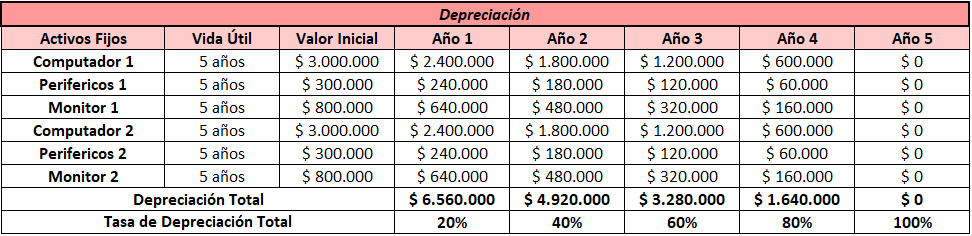
\includegraphics[width=13cm]{Imagenes/Depreciacion.png}
	\label{Depreciacion}
\end{table}